\documentclass[12pt,a4paper]{article}

\usepackage{anyfontsize}
\usepackage{graphicx}

%package for list formatting (ordered) if we add [a.]
\usepackage{enumerate}
%package for graphics or include images
\usepackage{graphicx}
\usepackage{float} %to place image forcefully there
\usepackage{pdfpages}
\usepackage{subcaption,caption}
\usepackage[hidelinks]{hyperref}

%for times new roman font
\usepackage{times,mathptmx}


%package for margins
\usepackage[outer=1.25in,inner=1.5in,top=1in,bottom=1in,headheight=0.5in,footskip=0.5in]{geometry}
%better to use outer and inner beacause while printing book then right and left margin will not be good , So, inner margin 


\begin{document}
	\pagenumbering{roman}
	
	
\begin{titlepage}
	
	\newcommand{\HRule}{\rule{\linewidth}{0.3mm}}
	\centering
	\vfill
	
\includegraphics[width=50mm]{images/tu.jpg}\\[0.75cm]
	\textsc{\Large \bfseries  TRIBHUVAN UNIVERSITY}\\[0.25cm] % Name of your university/college
	\textsc{\Large \bfseries INSTITUTE OF ENGINEERING}\\[0.25cm]
	\textsc{\Large \bfseries  PULCHOWK CAMPUS}\\
	\vfill
	\large {A PROJECT PROPOSAL ON }\\
	\Large \textbf{BAAL ARJUN : A 2D ARROW SHOOTING GAME}
	\vfill
	%\large \textbf{Subject code} \\[0.2cm]
%	\bfseries
	\large
	Submitted by:\\
	\textbf{ANUJ SHRESTHA} (078BCT014)\\
	\textbf{ARISHA PRASAIN} (078BCT019)\\
	\textbf{AYUSH ADHIKARI} (078BCT024)\\[0.5cm]
	\vfill
	\large
	A PROJECT PROPOSAL TO THE DEPARTMENT OF ELECTRONICS AND COMPUTER
	ENGINEERING ON OBJECT ORIENTED PROGRAMMING APPLICATION USING
	C++
	\vfill
	SUBMITTED TO:\\
	\textbf{DEPARTMENT OF ELECTRONICS AND COMPUTER ENGINEERING}
	\\
	\vfill
	{\large \today}
	\vfill
\end{titlepage}

	
  	
  	
  	\newpage
\section*{ACKNOWLEDGEMENT}
\addcontentsline{toc}{section}{ACKNOWLEDGEMENT}

We would like to extend our sincere gratitude to our esteemed Lecturer, Mr. Daya Sagar Baral, for granting us the invaluable opportunity to undertake the project work on Object-Oriented Programming in C++. We express our heartfelt appreciation for his invaluable support and guidance, which played a crucial role in ensuring the success of this project. We would also like to express our deepest gratitude to the Department of Electronics and Computer Engineering at the Institute of Engineering, Pulchowk Campus, for providing us with the opportunity to collaborate on this endeavor. Additionally, we extend our thanks to our laboratory instructors for their guidance and support throughout our work in the computer lab.
\\\\
We are immensely thankful to all our friends who have contributed to the development of this project, and we sincerely appreciate their assistance. We welcome constructive criticism and recommendations in any form, and we assure you that they will be received with an open heart, valued, and duly acknowledged.

\vskip 8mm
\begin{flushleft}
	{\bf Authors:}
	\newline Anuj Shrestha
	\newline Arisha Prasain
	\newline Ayush Adhikari		
\end{flushleft}
  	

\newpage
\section*{ABSTRACT}
\addcontentsline{toc}{section}{ABSTRACT}

The principal aim of this project was to create a gaming program utilizing an Object-Oriented Programming language, C++. Within the scope of this project, we crafted a 2D game centered around arrow-based combat using the Simple and Fast Multimedia Library (SFML) to handle the graphical user interface. The underlying objective of developing this game also encompassed the insights into the world of game development.\\\\
Baal Arjun stands as a 2D, single-player computerized game. This game constitutes a simple two-dimensional rendition of a battlefield, presented from a top-down perspective. In this scenario, the player assumes the role of the character 'Arjuna' and engages in shooting arrows at adversaries and their cohorts. The initial three levels have been designed to function as a means of familiarizing the player with the game interface. Successful completion of each level hinges upon the player's ability to triumph over the adversaries prior to succumbing to their own defeat. Should the player emerge successful in this endeavor, they attain victory; conversely, failure to do so results in defeat.\\\\
\textit{Keywords: Baal Arjun, SFML, Object-Oriented Programming, C++}
  \newpage
  \tableofcontents
  	
%  	\newpage
%  	{
%  		\setlength{\parskip}{0em}
%  		\renewcommand\contentsname{TABLE OF CONTENTS}\\[0.5cm] % This will change heading text
%  		\tableofcontents 
%  	   % \addcontentsline{toc}{section}{TABLE OF CONTENTS}
%  	}
  	
  	
  	
  	\newpage
\pagenumbering{arabic}
\section{OBJECTIVES}
The primary objective of this project is to facilitate the practical application of the Object-Oriented Programming (OOP) model using the well-established and effective programming language, C++. The key objectives pertaining to the development of this project are outlined as follows:

\begin{enumerate}
	\item To gain a comprehensive understanding of the Object-Oriented Programming paradigm, encompassing its principles and successfully implementing them in the project.
	\item To explore the fundamental as well as advanced features offered by C++.
	\item To acquire knowledge and proficiency in designing custom header files, thereby familiarizing ourselves with the concepts of modularity and reusability.
	\item To acquire a foundational understanding of game development and testing, with a specific focus on the development of game.
	\item To become acquainted with graphics libraries such as SFML, enabling the design and implementation of a user-friendly user interface (UI).
	\item To develop a program that exhibits high performance and efficiency, taking the factors such as memory management, time constraints, algorithmic complexity, and optimal resource utilization into consideration. 
	\item To enhance our abilities in teamwork and collaborative communication, fostering effective cooperation among project members.
	
\end{enumerate}

By pursuing these objectives, we aim to gain practical knowledge and skills in OOP principles, C++ programming, modular design, game development practices, UI design, and optimization techniques. Moreover, this project serves as an opportunity to strengthen our collaborative abilities, enhancing our team dynamics and communication skills.

  	\newpage
\pagenumbering{arabic}
\section{INTRODUCTION}
Baal Arjun is a 2D arrow shooting game that takes inspiration from the esteemed character Arjuna in the epic Mahabharata, who is widely regarded as the preeminent archer of that era. This game, known as "Baal Arjun," offers an engaging single-player experience, consisting of three chapters, each comprising numerous levels.\\\\
Within each level, the player navigates the screen and utilizes both the mouse and keyboard to precisely adjust the angle of the character named 'Arjun' in order to strike the target. The angle and position of the character can be modified until the left mouse button is clicked. Once the left button is released, the arrow swiftly propels toward the designated target coordinate. Initially, the player is allotted a limited number of arrows and possesses a finite life. With each successful hit on the target, the player's score increases. If the target is missed, the player continues playing the same level until all arrows are depleted. To successfully pass a level, all targets must be accurately hit within the designated time frame, subsequently unlocking the next level.\\\\
In the initial stages, the targets remain stationary, gradually transitioning into a non-stationary state as the levels progress, thus adding an element of challenge and dynamism to the gameplay.
\\
\vspace{1.5 cm}
\begin{figure}[h]
	
	\centering
	
\includegraphics[width = \textwidth]{sec/pdf/loading}
	\caption{Proposed Loading Screen}
\end{figure}

  	
\section{APPLICATION}
Our project involves developing an exciting game based on the character Arjun from Mahabharat. Players will control Arjun and use their mouse to shoot arrows at targets while moving in the game world.



 \subsection{User Engagement}
	We aim to create an engaging game that immerses players in the world of Arjun. By providing an enjoyable experience, we hope to entertain players and make them feel connected to the character and the epic.
	
 \subsection{Skill Development}
	The gameplay mechanics, such as arrow shooting and precision aiming, offer players the chance to improve their hand-eye coordination, concentration, and reflexes. These skills can be valuable not just in the game, but also in real-life situations.
	
 \subsection{Cultural Appreciation}
	Our game's theme, inspired by Mahabharat, aims to spark interest and curiosity among players who are fans of the epic or have an interest in Hindu mythology and culture. We want to contribute to cultural appreciation and raise awareness of this rich heritage.
	
 \subsection{Learning and Engagement with Mahabharat}
	Through the gameplay and accompanying content, we want to provide players with an opportunity to learn more about Arjun and his role in Mahabharat. By delving into the mythology, players can gain insights and develop a deeper understanding of the epic.

\subsection{ Entertainment Industry Impact}
	If our game gains popularity and positive reception, it could have an impact on the entertainment industry. It may inspire similar projects and encourage the exploration of Indian mythological themes in gaming, diversifying the offerings in the industry.



Our project aims to develop an immersive and enjoyable game centered around Arjun from Mahabharat. We want to provide players with an engaging experience, improve their skills, foster cultural appreciation, facilitate learning about Mahabharat, and potentially contribute to the broader landscape of the entertainment industry.

\pagebreak


\newpage
  	\section{LITERATURE REVIEW}
"Baal Arjun" stands as a captivating 2D arrow shooting game, deeply rooted in the narrative tapestry of the Mahabharata. In this innovative gaming venture, players assume the role of Arjun, embarking on a solitary quest to confront adversaries. The game's premise revolves around Arjun's adeptness at evading enemy arrows while expertly aiming and retaliating. By seamlessly blending cultural heritage with cutting-edge technology, "Baal Arjun" emerges as a conduit bridging the gap between tradition and modernity. While it is  a notable fact that there aren't many games that are based on the epic 'Mahabharata', this literature review critically examines the conceptualization and significance of "Baal Arjun" within the contemporary gaming landscape.


\subsection{Harmonizing Cultural Legacy with Technological Ingenuity}
In an era marked by technological advancement and cultural evolution, "Baal Arjun" masterfully harmonizes these seemingly disparate elements. By effortlessly infusing the theme of the Mahabharata, the game offers players an immersive experience that resonates with our profound Hindu heritage. This synthesis of cultural motifs underscores the visionary approach of "Baal Arjun", aligning with the insights of various authors, who champion digital platforms as potent vehicles for cultural preservation.

\subsection{Elevating Cultural Representation in Gaming}
Distinctive in its approach, "Baal Arjun" addresses a conspicuous gap in contemporary gaming – the nuanced representation of Hindu culture. In a milieu replete with diverse gaming themes, the game's embrace of our cultural nuances is pioneering. Its innovative narrative resonates with the propositions that gaming platforms serve as conduits for cultural appreciation and understanding.

\subsection{Cultivating Educational Exploration}
Beyond its entertainment quotient, "Baal Arjun" presents an edifying dimension, offering players a conduit for cultural learning. By immersing players in the Mahabharata's essence and embodying Arjun's valor, the game subtly imparts historical and mythological knowledge. This resonates with the educational potential of games underscored by Gee (2003)*, where games serve as interactive mediums for assimilating intricate narratives and honing problem-solving skills.

\subsection{Navigating Challenges and Reaping Rewards}
Arjun's journey, interwoven with evasion and precision shooting, mirrors the rigors of real-life challenges. The gameplay is intrinsically aligned with Csikszentmihalyi's ** concept of "flow," wherein challenges are synchronized with a player's proficiency, engendering immersive experiences. The successful navigation of these challenges begets a sense of achievement, spurring players to persevere and excel.

\subsection{A Paradigm Shift in Gaming}
"Baal Arjun" transcends the confines of conventional gaming, assuming the role of a transformative force that amalgamates culture and technology. As it propels a digital resurgence of our cultural heritage, the game endeavors to captivate players while fostering cultural resonance. In a gaming milieu characterized by innovation and diversity, "Baal Arjun" aspires to carve a distinctive niche, poised at the crossroads of tradition and the digital age.

 

In conclusion, "Baal Arjun" symbolizes a unique symbiosis between cultural heritage and technological prowess. By offering an interactive platform steeped in Hindu traditions, the game endeavors to enthral players while fostering cultural reverberations. Within a dynamic gaming landscape characterized by ceaseless evolution, "Baal Arjun" assumes an unprecedented role, standing as a trailblazer in the realm of cultural gaming exploration.
\\\\\\
* - "Gee (2003)" refers to the real scholar James Paul Gee and his work "What Video Games Have to Teach Us About Learning and Literacy" published in 2003. In the context of the literature review, Gee's ideas are referenced to support the concept that games can serve as interactive mediums for education and learning. His work is often cited in discussions about the educational potential of video games.
\\\\
** - Mihaly Csikszentmihalyi is a psychologist known for his work on the concept of "flow." Flow is a state of complete immersion and engagement in an activity, where challenges are balanced with one's skill level, resulting in a highly focused and enjoyable experience.

\newpage
 % 	\section{EXISTING SYSTEM}
hi

\newpage
  	
\section{METHODOLOGY}
To complete our project, we followed the following methods:


	\subsection{Research and Planning} 
	\begin{enumerate}
		\item  Conduct research on various aspects of game development, including features, fundamental requirements, and tools required.
		\item Familiarize ourselves with the necessary libraries and divide the work among the team members.
		\item Develop comprehensive coding guidelines to ensure self-documenting code.
		
	\end{enumerate}
	\subsection{ Algorithm Design }
	\begin{enumerate}
		
		\item Design the algorithm and create a flowchart based on the gathered rules and information. 
		\item Develop a basic prototype for testing purposes, using the console.
		
		
	\end{enumerate}
	
 \subsection{Sources}
	Utilize the following sources as references to support our project:
	\begin{enumerate}
		
		\item Documentation for SFML.
		\item Concepts of object-oriented programming (OOP) and C++ programming from college courses, online references, books, etc.
		
		
	\end{enumerate}
	
	\subsection{ Game Design}
	
	\begin{enumerate}
		
		\item Implement the code using an object-oriented programming (OOP) paradigm. 
		\item Use Simple and Fast Multimedia Library to create build the game.
		\item Choose Visual Studio as our Integrated Development Environment (IDE) and visual c++ as the compiler in the Windows Operating System.
		\item Manage our code using GitHub for version control.
		
	\end{enumerate}
	
 \subsection{Maintenance}
	Regularly maintain the project by following these procedures:
	\begin{enumerate}
		
		\item Corrective maintenance:
		\begin{itemize}
			\item Compile and check specific parts of the code for potential bugs and errors, fixing them as necessary.
		\end{itemize}
		
		\item  Preventive maintenance:
		\begin{itemize}
			
			\item Identify errors and take measures to avoid them during runtime and the development cycle.
			\item Comment and document the source code thoroughly and back it up to prevent potential data loss.
			
			
		\end{itemize}
	\end{enumerate}

	\subsection{Testing and Debugging}
	\begin{enumerate}
		
		\item Develop a minimum viable product sample for testing and debugging purposes.
		\item Conduct frequent testing and debugging to add features and make necessary edits to the project code based on our requirements and capabilities.
		
	\end{enumerate}
	\subsection{ Documentation}
	\begin{enumerate}
		\item Ensure comprehensive documentation of the app, including the addition of copyright licenses.
		\item Ship the completed app with the accompanying documentation.
	\end{enumerate}


\newpage



  	\section{IMPLEMENTATION}


	 \subsection{Approach}
	
		The implementation of our project was structured into several distinct phases, each centered around specific gameplay mechanics, visual design, and user interaction. This approach facilitated a continuous process of refinement and enhancement as we progressed.
	
	 \subsubsection{Tools and Technologies}
		\begin{enumerate}
			\item Programming Languages
			
					We selected C++ as the primary programming language for our game's development. Its exceptional speed and object-oriented nature significantly streamlined the process of coding the game's mechanics.
			\item Libraries
			
					For multimedia and graphics user interface implementation, we harnessed the capabilities of the SFML library. Chosen for its user-friendly syntax and comprehensive toolkit, SFML provided us with all the essential resources required for effective game development.
			
		\end{enumerate}
	
	\subsubsection{System Architecture and Design}
	
		The architecture of "Baal Arjun" was thoughtfully structured to ensure both flexibility and scalability. Key components encompassed in this architecture include:
		
		\begin{enumerate}
			\item Player Controller:
				Responsible for managing player inputs, character movement, and shooting mechanics.
			
			\item Enemy Automation:
				Incorporating dynamic enemy movement and     arrow-shooting behavior.
			
			\item Collision Detection: 
				 Overseeing accurate collision detection between arrows, characters, and the game environment.
				 
			\item Level Implementation:
					Designing and integrating game levels to ensure a dynamic player experience.
			\item User Interface (UI):
					 Displaying essential in-game information such as health, arrow count, and visual elements for enemies and player arrows.
			\item Sound Implementation:
					Enriching gameplay through auditory elements.
			
		\end{enumerate}
		
 \subsubsection{Code Development}
			
			The foundational gameplay mechanics were meticulously developed, spanning aspects like player movement, arrow physics, enemy behavior, shooting mechanisms, collision detection, and the implementation of diverse game levels. Algorithmic solutions were devised for trajectories of normal and Sudarshan arrows, each rigorously tested and refined. Emphasis was placed on crafting self-documented code, achieving modularity for code reusability.
	
	 \subsubsection{Resource Collection}
	
	 		Resources such as images, sounds, and fonts were thoughtfully curated from online sources. Furthermore, Adobe Illustrator was leveraged to modify these resources to align precisely with our project's creative vision.
	 		
	 		
	  \subsubsection{Integration and Testing}
	 
	 		The integration process commenced by combining shooting algorithms with collision detection algorithms, subjecting them to comprehensive testing to ensure their seamless functionality. Concurrently, the graphical user interface (GUI) underwent development. Eventually, the GUI and game logic converged into the final cohesive product. A testing phase was initiated, involving friends as testers who aided in identifying and rectifying any bugs encountered.
	 		
	 \subsubsection{Version Control and Collaboration}
	 
	 		To facilitate seamless collaboration, GitHub served as our chosen version control system. Regular code synchronization was achieved through Git, ensuring that contributions from all team members were harmoniously integrated.
	 		


This comprehensive implementation phase not only actualized our project but also exemplified our commitment to precision, collaboration, and the realization of an engaging gaming experience.

\newpage
\subsection{Flow Chart}

\vspace{2cm}
\begin{figure}[h]
	
	\centering
	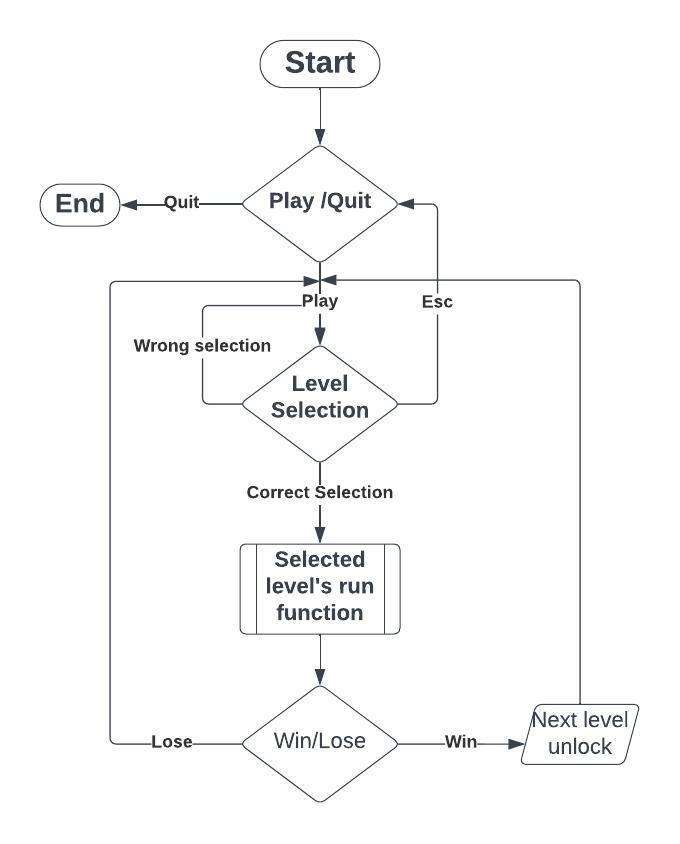
\includegraphics{sec/pdf/flowchart}
	\caption{Flow Chart}
\end{figure}

\newpage
\subsection{Block Diagram}

\vspace{2cm}
\begin{figure}[h]
	
	\centering
	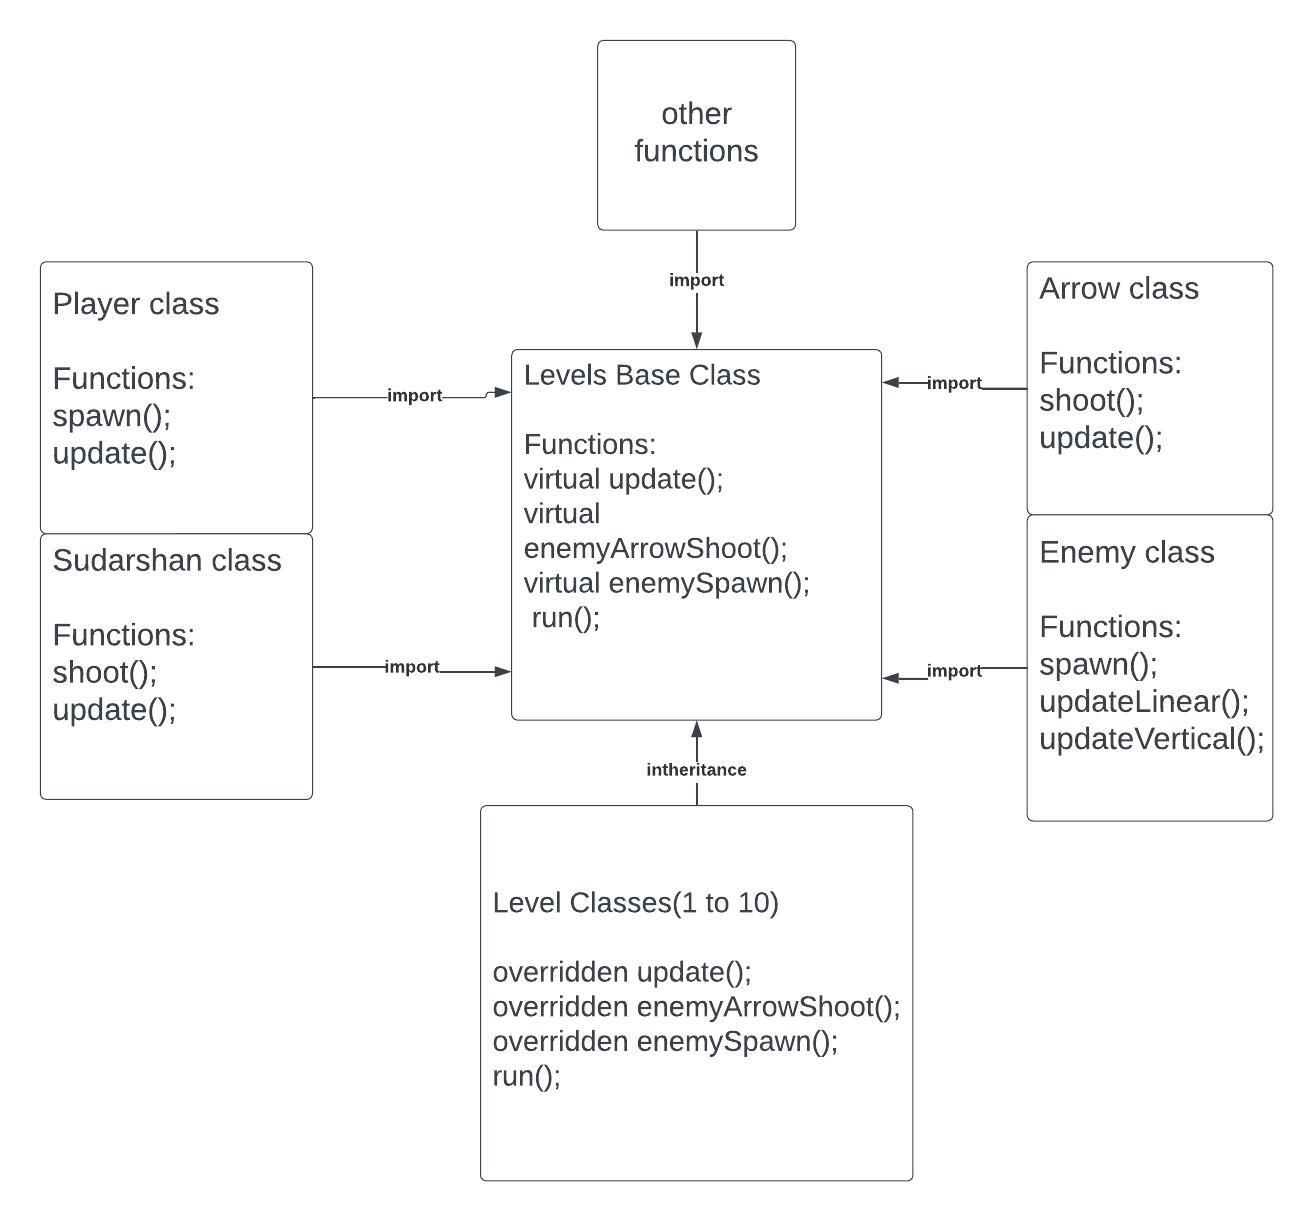
\includegraphics[width = \textwidth]{sec/pdf/blockDiagram}
	\caption{Generalized Block Diagram}
\end{figure}

\newpage
\subsection{Game Pictures}
\vspace{2cm}
\begin{figure}[h]
	
	\centering
	
\includegraphics[width = \textwidth]{sec/pdf/main}
	\caption{Main Screen}
\end{figure}
\vspace{2cm}
\begin{figure}[h]
	
	\centering
	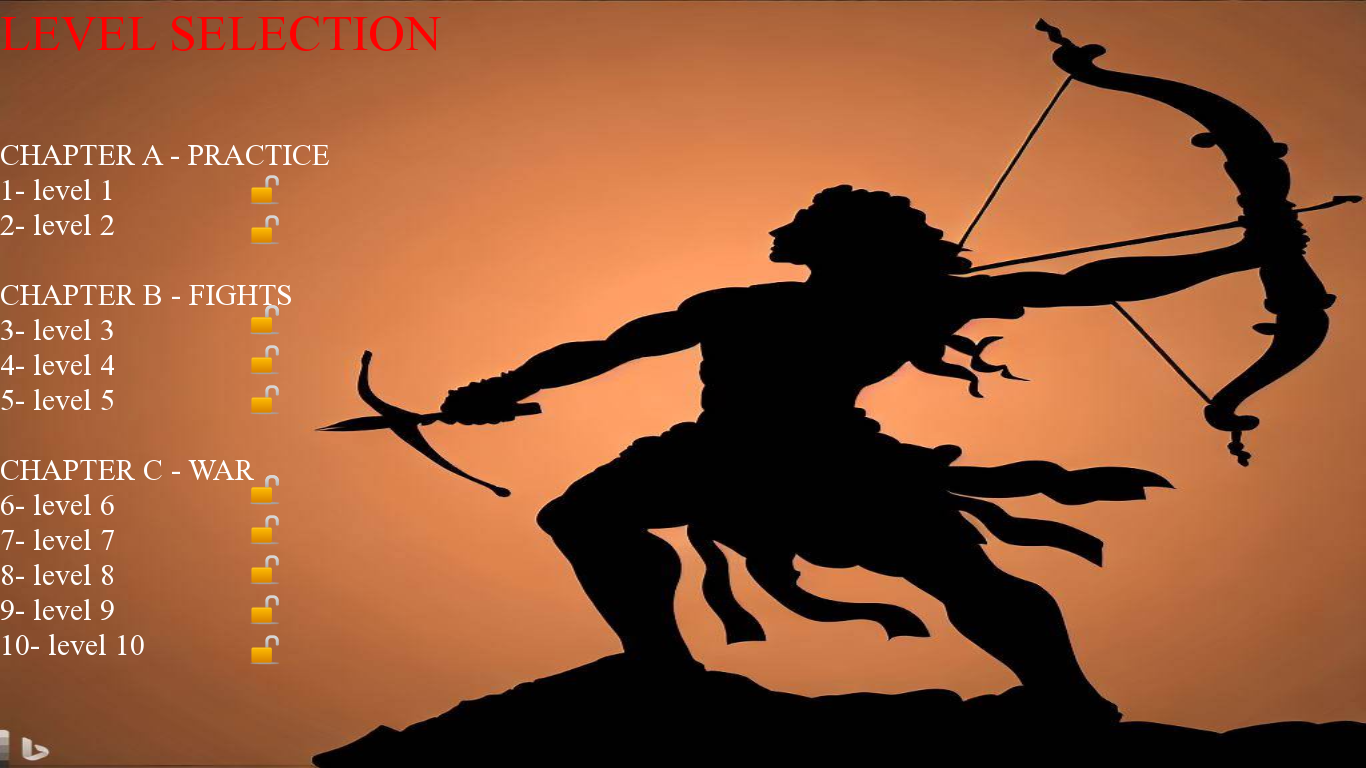
\includegraphics[width = \textwidth]{sec/pdf/chapters}
	\caption{Level Selection Screen}
\end{figure}

\newpage
\begin{figure}[h]
	
	\centering
	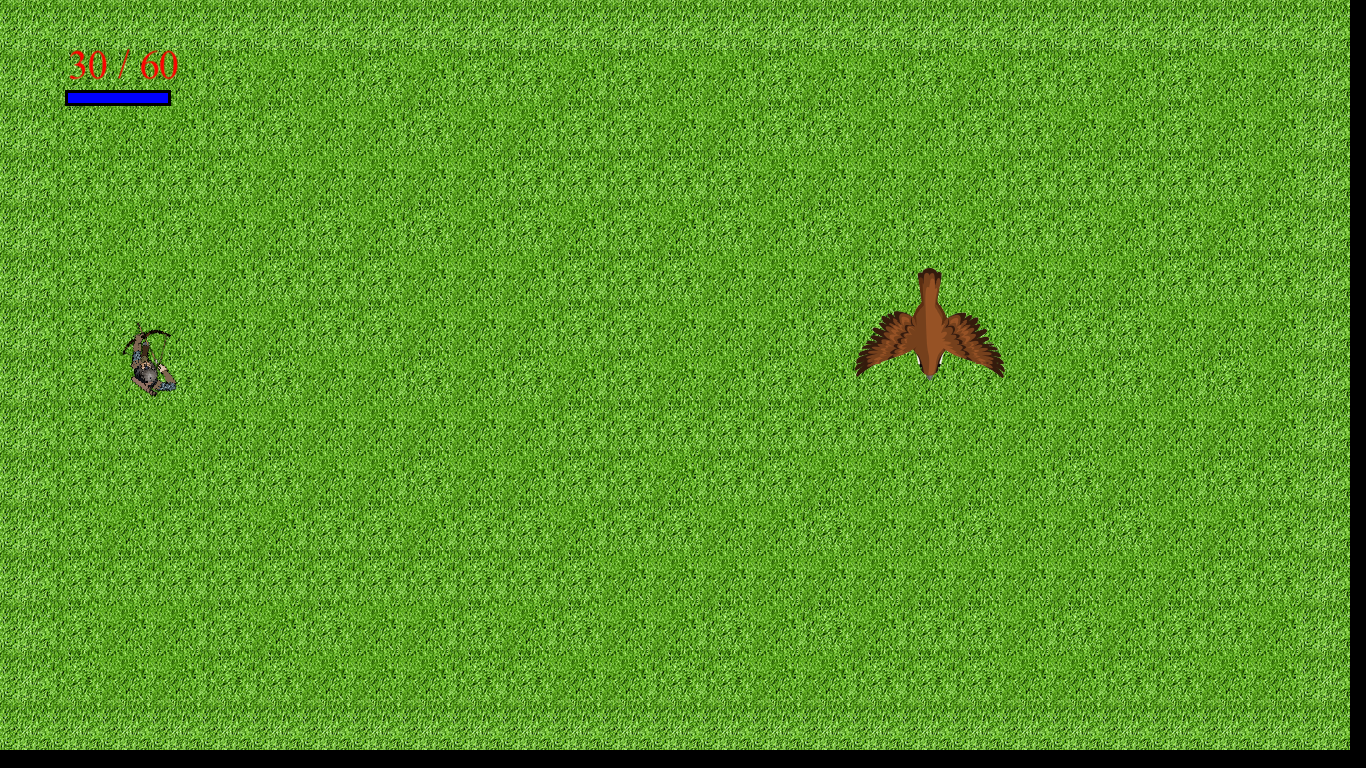
\includegraphics[width = \textwidth]{sec/pdf/level2}
	\caption{Level 2}
\end{figure}
\vspace{2cm}
\begin{figure}[h]
	
	\centering
	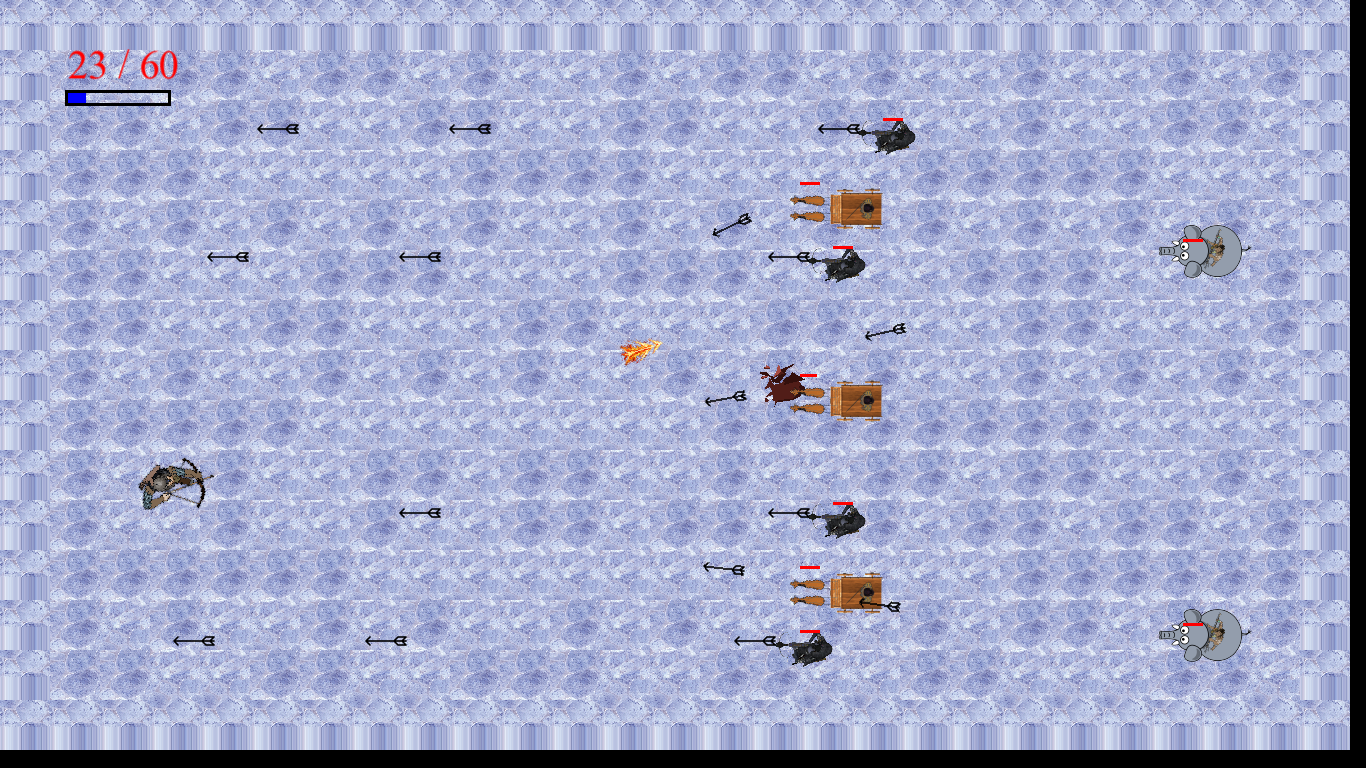
\includegraphics[width = \textwidth]{sec/pdf/level 7}
	\caption{Level 7}
\end{figure}
\newpage
\vspace{2cm}
\begin{figure}[h]
	
	\centering
	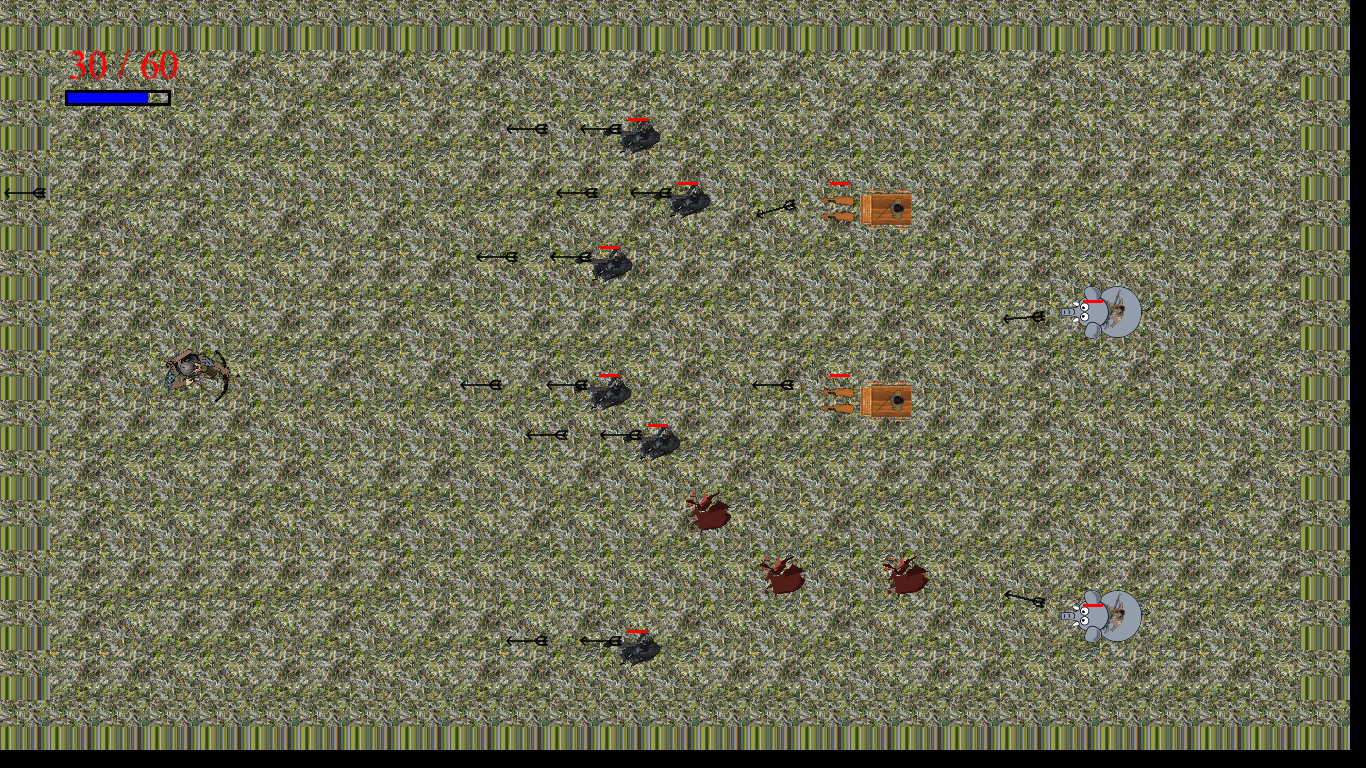
\includegraphics[width = \textwidth]{sec/pdf/level 8}
	\caption{Level 8}
\end{figure}

\vspace{2cm}
\begin{figure}[h]
	
	\centering
	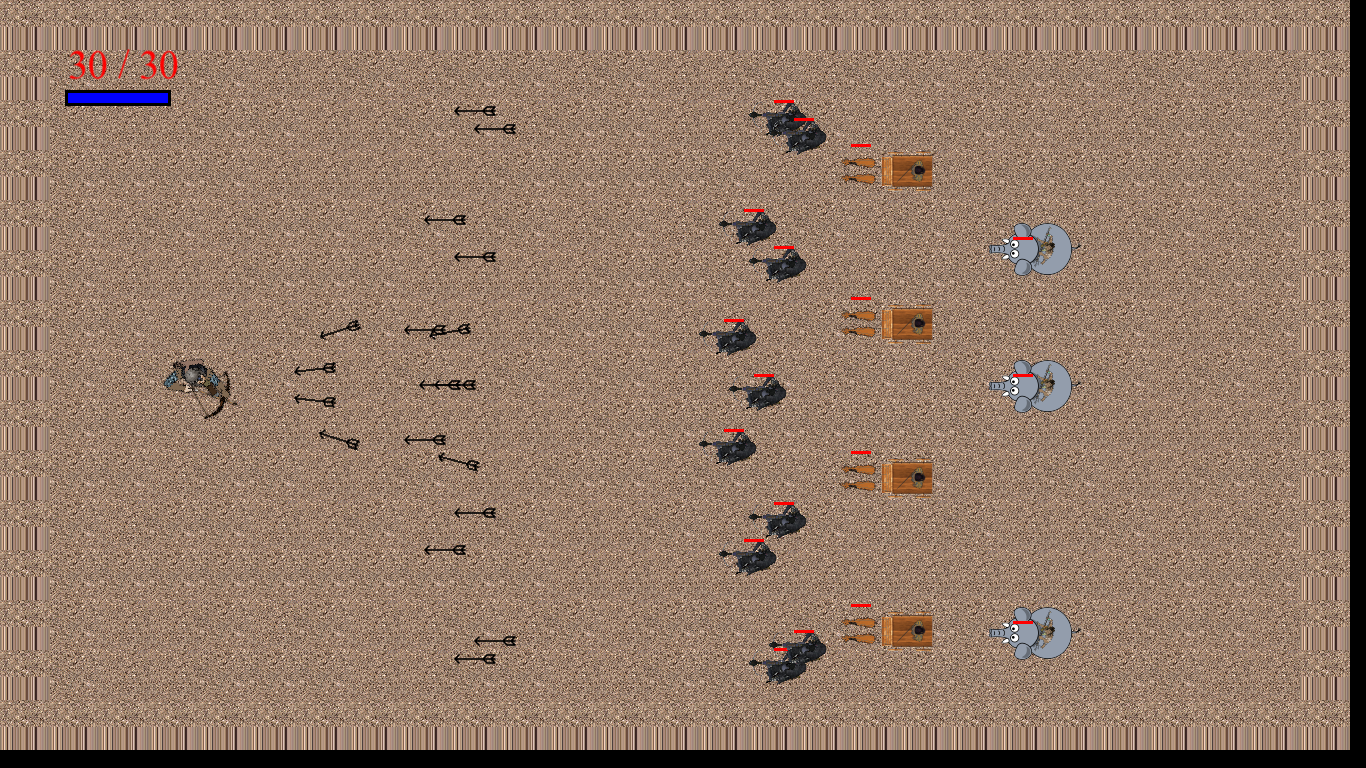
\includegraphics[width = \textwidth]{sec/pdf/level 9}
	\caption{Level 9}
\end{figure}




\newpage
  	\section{RESULTS}
The implementation of Object Oriented Programming concept using C++, the development of GUI environment employing the Safe and Fast Multimedia Library (SFML), the application of mathematical formulas and algorithm to ensure seamless and glitchfree gaming experience and the contionus efforts involved in writing, debugging and testing the program has resulted in a functional product, 'Baal Arjun' - a 2D arrow shooting game. While always being openminded for future enhancements and constructive crticism, we believe, with the successful creation of this playable game, the objectives of this project have been duly achieved.

\newpage
  	\section{PROBLEM FACED AND SOLUTIONS}
Problem Faced and solution:

\begin{enumerate}
	\item Code Manageability
	
	The use of Object Oriented programming helped us in dividing the code into multiple parts(header and cpp files) and manageable chunks. Navigating between certain parts of the code often and finding specific lines were tedious due to the sheer volume of the code spread throughout 25+ header and cpp files.
	
	This problem was solved by using naming the files, classes, objects, variables and functions with relevant names. The naming was greatly assisted by SFML library declared variable and function names. Proper Comments were mentioned in each and every section of code which in turn, increased code readability as well as facilitated code manageability.
	
	
	\item  Arrow Overriding
	While we were satisfied by SFML library defined functions, one of the unexpected problems faced was - whenever a new arrow was shot by enemy, the previous arrow simply disappeared from screen. This ensured undue immunity to player which contradicted the motive of the game.
	
	The solution entailed passing the count of arrows using a "pass by reference" mechanism, thereby enabling accurate tracking and management of all arrows within the game environment.
		
	\item Debugging and Updating
	A true developer knows how much debugging and testing goes on, even while writing a relatively simple code. As such, we were not immune to this phenomena, specially in each level while setting the attributes of  enemy ie , the position of every enemies and their speed. Similar problem was faced while writing the level selection and play/quit code.
	
	This problem was solved by intensively following hit and trial method. All of the code was rigorously tested so as to minimize errors and create smooth and seamless gaming experience.
	
	\item Lack of Appropriate Images
	Since the visual orientation of the game was top view, there were not a lot of images that followed the rather unconventional view. Most images we found were either front view or angular view, but as we choose top down view due to its benefit that both x and y axis along with rotation could be involved, the overall graphical aesthetics of the game was compromised. Even after spending a lot of time searching images such as (warrior from top view, horse carriage from top view, etc. ) and free tokens in AI image generators, the results were not satisfactory.
		
\end{enumerate}



This problem was solved by selecting the image which best fit our requirement and image manipulation (such as combining top view of horses, top view of empty carriage , and top view of a standing warrior to make top view of a warrior in a horse carriage ). 
\newpage
  	\section{LIMITATIONS AND FUTURE ENHANCEMENTS}

\subsection{Limitations}
\begin{enumerate}
	\item The game doesn't show the player's score and highest achieved score.
	\item Both easy and hard levels have the same number of arrows, which might not suit the difficult level.
	
	\item The game lacks a coherent storytelling and instructional guide for players.
	\item There are no shields or protective mechanisms for the player-character.
	\item The game lacks methods to restore the player's health or replenish arrows during gameplay.
	\item The absence of a comprehensive reward system, such as earning coins.
	\item The game lacks improvements or upgrades for the player's bow and arrows.
	\item The graphical user interface (GUI) is not fully immersive
\end{enumerate}



\subsection{Future Enhancements}
\begin{enumerate}
	\item New types of arrows:
	 Additional arrow varieties could be introduced, enhancing gameplay diversity and strategy. 
	\item Graphics improvement:
	 Enhancements to the game's visual elements could lead to a more immersive and appealing user experience.
	\item More difficult levels:
	 The incorporation of increasingly challenging levels would provide players with greater engagement and progression challenges.
	\item Avatar customization: 
	The addition of avatar customization options would allow players to personalize their in-game characters.
	\item  Health increment mechanism:
	 Implementing a mechanism to increase in-game health could extend gameplay and strategic options. This could be done by placing health boosters at random positions on the gamescreen.
	\item Reward system:
	 A structured reward system could motivate players by recognizing their accomplishments and fostering a sense of achievement. This may be achieved by rewarding the player with coins, which can be used to restore in-game health, and to purchase new and more powerful bows and arrows.
	\item Shield feature:
	 Introducing a shield mechanic could introduce a new layer of gameplay tactics and defensive strategies. This could also be done by placing shield enablers at random position in player's arena, which activates shield for a limited time period.
	\item  Enriched storytelling:
	 Enhancing the narrative elements could deepen player immersion and emotional investment in the game's world using voice records or AI generated voice of the story.
\end{enumerate}


\newpage
  	\section{CONCLUSION AND RECOMMENDATIONS}
thisis conclud


\newpage
  	\section{REFERENCES}


 \hspace{0.65cm}[1] Baral, D S.(2018).Secrets of Object Oriented Programming in C++\\
 
 [2] https://www.sfml-dev.org/documentation/2.6.0/\\
 
 [3] Stroustrup, B.(2013).The C++ Programming Language, 4th edition\\
 
\newpage
  	
  	
  
  
  
  
	
\end{document}


